% Setup -------------------------------

\documentclass[a4paper]{report}
\usepackage[a4paper, total={6in, 10in}]{geometry}
\setcounter{secnumdepth}{3}
\setcounter{tocdepth}{3}

\usepackage{hyperref}
\usepackage{indentfirst}

\usepackage{fancyvrb}
\usepackage{xcolor}

\usepackage{graphicx}

\usepackage{float}

% Encoding
%--------------------------------------
\usepackage[T1]{fontenc}
\usepackage[utf8]{inputenc}
%--------------------------------------

% Portuguese-specific commands
%--------------------------------------
\usepackage[portuguese]{babel}
%--------------------------------------

% Hyphenation rules
%--------------------------------------
\usepackage{hyphenat}
%--------------------------------------

% Capa do relatório

\title{
	Gestão de Grandes Conjuntos de Dados
	\\ \Large{\textbf{1º Trabalho Prático}}
	\\ -
	\\ Mestrado em Engenharia Informática
	\\ Universidade do Minho
}
\author{
	\begin{tabular}{ll}
		\textbf{Grupo nº 8}
		\\
		\hline
		PG41080 & João Ribeiro Imperadeiro
        \\
		PG41081 & José Alberto Martins Boticas
		\\
        PG41091 & Nelson José Dias Teixeira
        \\
        PG41851 & Rui Miguel da Costa Meira
	\end{tabular}
}

\date{\today}

\begin{document}

\begin{titlepage}
    \maketitle
\end{titlepage}

% Índice

\tableofcontents
\listoffigures

% Introdução

\chapter{Introdução} \label{ch:Introduction}
\large {
	Neste trabalho prático é requerida a concretização e avaliação experimental de tarefas de armazenamento e processamento de dados através do uso das ferramentas computacionais \textit{Hadoop HDFS}, \textit{HBase} e \textit{Hadoop MapReduce}.
	Por forma a realizar estas tarefas, são utilizados os dados públicos do \textit{IMDB}, que se encontram disponíveis em: 
	\begin{center}
		\textit{\url{https://www.imdb.com/interfaces/}}
	\end{center}

	Ao longo deste documento vão também ser expostos todos os passos tomados durante a implementação das tarefas pedidas neste projeto, incluindo as decisões tomadas pelos elementos deste grupo a nível de algoritmos e parâmetros de configuração.
	Para além disso são ainda apresentadas todas as instruções que permitem executar e utilizar corretamente os programas desenvolvidos.
	Por fim, na fase final deste manuscrito, são exibidos os objetivos atingidos após a realização das tarefas propostas.

	De salientar ainda que durante os capítulos que se seguem são identificadas algumas alternativas para concretizar as tarefas indicadas neste trabalho prático.
}

\chapter{Implementação} \label{ch:Implementation}
\large {
	Para a realização com sucesso deste trabalho, é solicitada a elaboração de duas tarefas, sendo elas:
	\begin{enumerate}
		\item Carregar os dados do ficheiro \textit{"title.basics.tsv.gz"} para uma tabela \textit{HBase};
		\item Utilizando a tabela \textit{HBase} do ponto acima e os restantes ficheiros presentes no \textit{dataset} mencionado no capítulo anterior, computar os dados necessários para apresentar para cada ator uma página. Esta última deve conter:
		\begin{itemize}
			\item nome, datas de nascimento e morte;
			\item número total de filmes em que participou como ator;
			\item títulos dos três filmes com melhor cotação em que participou.
		\end{itemize}
		Estes dados devem ser armazenados numa tabela \textit{HBase}.
	\end{enumerate}
	
	Nas próximas secções são evidenciadas as implementações para cada uma destas tarefas bem como algumas sugestões alternativas que poderiam ser tomadas em consideração.
	
	\section{Arranque do \textit{cluster}} \label{sec:Cluster}
		À semelhança do que foi realizado no guião nº 4 desta unidade curricular, os elementos deste grupo utilizaram a plataforma \textit{Hadoop deployment} com recurso à ferramenta \textit{docker-compose}. Este utensílio computacional encontra-se disponível em:
		\begin{center}
			\textit{\url{https://github.com/big-data-europe/docker-hbase}}
		\end{center}

		De forma a proceder ao arranque do \textit{cluster} contido neste repositório basta simplesmente invocar a seguinte instrução:
		\begin{figure}[H]
			{
				\color{teal}
				\begin{verbatim}
				       docker-compose -f docker-hbase/docker-compose-distributed-local.yml up
				\end{verbatim}
			}
			\caption{Arranque do \textit{cluster}}
            \label{fig:1}
		\end{figure}

		Após a execução desta instrução, o \textit{cluster} que será utilizado neste projeto encontra-se corretamente instanciado e, como tal, pode-se proceder à realização das tarefas mencionadas anteriormente.

	\section{1ª Tarefa} \label{sec:Task1}
		Após descarregar o ficheiro \textit{"title.basics.tsv.gz"} presente na hiperligação do capítulo anterior, os elementos que compõem este grupo optaram por descompactá-lo, de forma a obter o mesmo no formato \textit{.tsv}.
		A tomada desta decisão deve-se ao facto de este último permitir a partição de dados (isto é, potencia o \textbf{paralelismo}), ao contrário do formato \textit{.gz} (\textit{gzip}). Para além disso, não é necessário descompactar aquando da sua utilização. Para além destes dois formatos, havia ainda a hipótese de utilizar o formato \textit{.bz2} (\textit{bzip2}), que, apesar de ser mais rápido e eficiente que o \textit{.gz}, não se compara com a ausência de descompressão do \textit{.tsv}.
		Mostra-se na seguinte figura a instrução associada à descompressão do ficheiro \textit{"title.basics.tsv.gz"}:
		\begin{figure}[H]
			{
				\color{teal}
				\begin{verbatim}
                            gzip -d title.basics.tsv.gz
				\end{verbatim}
			}
			\caption{1ª Tarefa - Conversão do ficheiro \textit{"title.basics.tsv.gz"} para o formato \textit{.tsv}}
            \label{fig:2}
		\end{figure}

		Antes de observar os passos relativos à realização desta tarefa, passos esses que se encontram explicitamente indicados nos próximos subcapítulos, é importante salientar que a execução das soluções elaboradas nas secções \hyperref[subsec:Task1-1]{2.2.1} e \hyperref[subsec:Task1-3]{2.2.3} são efetuadas com recurso a um ficheiro denominado por \textit{Dockerfile}.
		De forma a entender melhor a configuração do mesmo, revela-se a seguir o seu conteúdo:
		\begin{figure}[H]
			{
				\color{teal}
				\begin{verbatim}
					   FROM bde2020/hadoop-base
					   COPY target/TP1-1.0-SNAPSHOT.jar /
					   ENTRYPOINT ["hadoop", "jar", "/TP1-1.0-SNAPSHOT.jar", "ClassName"]
				\end{verbatim}
			}
            \caption{1ª Tarefa - \textit{Dockerfile}}
            \label{fig:3}
        \end{figure}
        
        Após esta observação, indica-se ainda as opções adotadas para a execução do ficheiro \textit{Dockerfile} com o intuito de garantir uma execução válida das soluções implementadas:
		\begin{figure}[H]
			{
				\color{teal}
				\begin{verbatim}
					   --network docker-hbase_default
					   --env-file ../docker-hbase/hadoop.env
					   --env-file ../docker-hbase/hbase-distributed-local.env
				\end{verbatim}
			}
			\caption{1ª Tarefa - \textit{Dockerfile} - Opções de execução}
			\label{fig:4}
        \end{figure}
		
		\subsection{Criação da tabela \textit{HBase}} \label{subsec:Task1-1}
		De forma a criar a tabela \textit{HBase} intrínseca a esta tarefa, foi implementada uma classe \textit{Java}, \textbf{\textit{CreateTableMovies}}, que, após conectar-se com a base de dados não relacional \textit{HBase}, trata da sua criação e configuração.
		Durante esse processo, é produzida apenas uma família de colunas, intitulada \textbf{\textit{details}}, onde será armazenada toda a informação associada aos dados do ficheiro \textit{"title.basics.tsv.gz"}.

		De notar também que se atribuiu o nome \textbf{\textit{movies}} à tabela gerada, tal como o nome da classe \textit{Java} transparece.

		Foi também criada uma classe \textit{Java} adicional, \textbf{\textit{DeleteTableMovies}}, que trata de eliminar a tabela descrita anteriormente.
		Esta foi desenvolvida com o intuito de remover a tabela em causa caso esta deixe se ser necessária no futuro.
        
        Apresenta-se de seguida o modelo da tabela \textit{HBase} pretendido para a concretização desta tarefa:
        \begin{figure}[H]
            \centering
            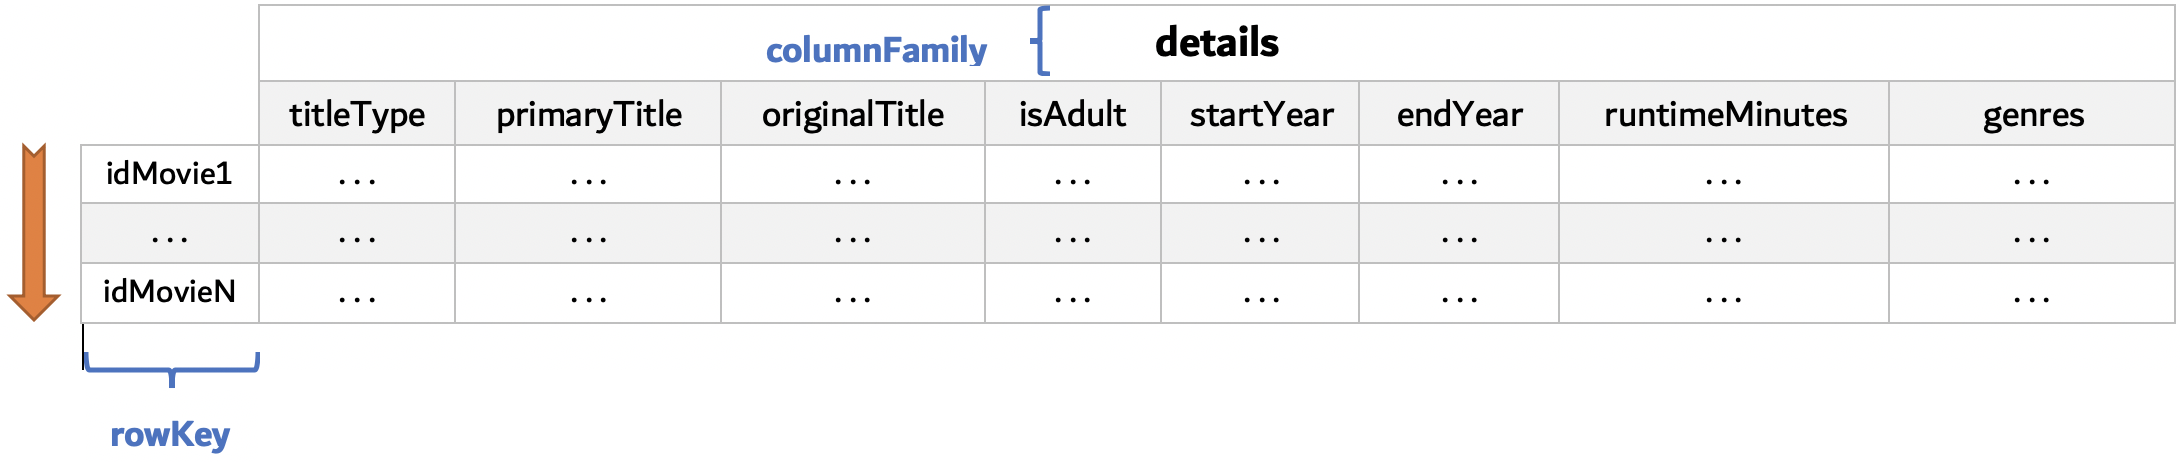
\includegraphics[width=1.0\textwidth]{Imagens/1ª Tarefa - Tabela Hbase.png}
            \caption{1ª Tarefa - Modelo da tabela \textit{HBase "movies"}}
            \label{fig:5}
        \end{figure}

			\subsubsection{Alternativa}
			Uma possibilidade válida para realizar todo o processo associado à criação da tabela requerida seria utilizar a \textit{HBase shell} de forma direta.
			Exibem-se de seguida as respetivas instruções:
			\begin{figure}[H]
				{
					\color{teal}
					\begin{verbatim}
					   docker run -it
					              --network docker-hbase_default
					              --env-file docker-hbase/hbase-distributed-local.env
					              bde2020/hbase-base hbase shell
					\end{verbatim}
				}
				\caption{1ª Tarefa : Alternativa - Acesso à \textit{HBase shell}}
				\label{fig:6}
			\end{figure}

			\begin{figure}[H]
				{
					\color{teal}
					\begin{Verbatim}[commandchars=\\\{\}]
                  \textcolor{orange}{hbase(main):001:0>} create "movies", "details"
					\end{Verbatim}
				}
				\caption{1ª Tarefa : Alternativa - Criação da tabela \textit{HBase "movies"}}
				\label{fig:7}
			\end{figure}
			
			Quanto à remoção da mesma tabela, à semelhança do procedimento tomado para a sua criação, adota-se a estratégia de usufruir explicitamente o mecanismo disponibilizado pela \textit{HBase shell}:
			\begin{figure}[H]
				{
					\color{teal}
					\begin{Verbatim}[commandchars=\\\{\}]
                        \textcolor{orange}{hbase(main):001:0>} disable "movies"
                        \textcolor{orange}{hbase(main):002:0>} drop "movies"
					\end{Verbatim}
				}
				\caption{1ª Tarefa : Alternativa - Remoção da tabela \textit{HBase "movies"}}
				\label{fig:8}
			\end{figure}

		\subsection{Transferência do ficheiro para a plataforma \textit{Hadoop HDFS}} \label{subsec:Task1-2}
		De maneira a proceder ao carregamento do ficheiro \textit{"title.basics.tsv"} para a plataforma \textit{Hadoop HDFS} existem duas possibilidades.
		Antes de exibir estas últimas alternativas, foi criada uma pasta na plataforma \textit{Hadoop HDFS}, denominada por \textit{data}, onde serão colocados todos os ficheiros de \textit{input} necessários.
		Exibe-se de seguida a instrução para tal efeito:
		\begin{figure}[H]
			{
				\color{teal}
				\begin{verbatim}
					   docker run --network docker-hbase_default
					              --env-file docker-hbase/hadoop.env
					              bde2020/hadoop-base hdfs dfs -mkdir /data
				\end{verbatim}
			}
			\caption{1ª Tarefa - Criação da pasta \texttt{data} na plataforma \textit{Hadoop HDFS}}
            \label{fig:9}
		\end{figure}

		Após a exposição deste comando, destacam-se nos próximos subcapítulos as duas alternativas mencionadas acima.

			\subsubsection{1ª Alternativa}
			Nesta possibilidade evidencia-se o campo \texttt{source} que corresponde à diretoria da pasta que contém o ficheiro \textit{"title.basics.tsv"}.
			Dito isto, apresenta-se agora a primeira alternativa:
			\begin{figure}[H]
				{
					\color{teal}
					\begin{verbatim}
					   docker run --network docker-hbase_default
					              --env-file docker-hbase/hadoop.env
					              --mount type=bind,source="/path/to/local/folder/data",target=/data
					              bde2020/hadoop-base hdfs dfs -put /data/title.basics.tsv /data
					\end{verbatim}
				}
				\caption{1ª Tarefa : 1ª Alternativa - Transferência do ficheiro \textit{"title.basics.tsv"} para a plataforma \textit{Hadoop HDFS}}
				\label{fig:10}
			\end{figure}

			\subsubsection{2ª Alternativa}
			Esta opção corresponde ao modo interativo de execução disponibilizado pela instrução \textit{docker run}.
			Uma vez feita esta observação, expõe-se a seguir a segunda alternativa:
			\begin{figure}[H]
				{
					\color{teal}
					\begin{verbatim}
					   docker run -it
					              --network docker-hbase_default
					              --env-file docker-hbase/hadoop.env
					              bde2020/hadoop-base bash

					   curl https://datasets.imdbws.com/title.basics.tsv.gz | gunzip |
					   hdfs dfs -put - hdfs://namenode:9000/data/title.basics.tsv
					\end{verbatim}
				}
				\caption{1ª Tarefa : 2ª Alternativa - Transferência do ficheiro \textit{"title.basics.tsv"} para a plataforma \textit{Hadoop HDFS}}
				\label{fig:11}
			\end{figure}

		\subsection{População da tabela \textit{HBase}} \label{subsec:Task1-3}
		Quanto à população da tabela criada previamente foi igualmente implementada uma classe \textit{Java} para o efeito, designada por \textbf{\textit{Movie2Details}}.
		Esta classe incorpora uma tarefa assente no paradigma \textit{MapReduce}, onde é apenas elaborada a fase de \textit{map}.
		Nessa mesma etapa é processada cada linha do ficheiro de \textit{input} presente na plataforma \textit{Hadoop HDFS} e, quando o tratamento estiver concluído, o resultado obtido é colocado na tabela \textit{movies}.
		
		\begin{figure}[H]
            \centering
            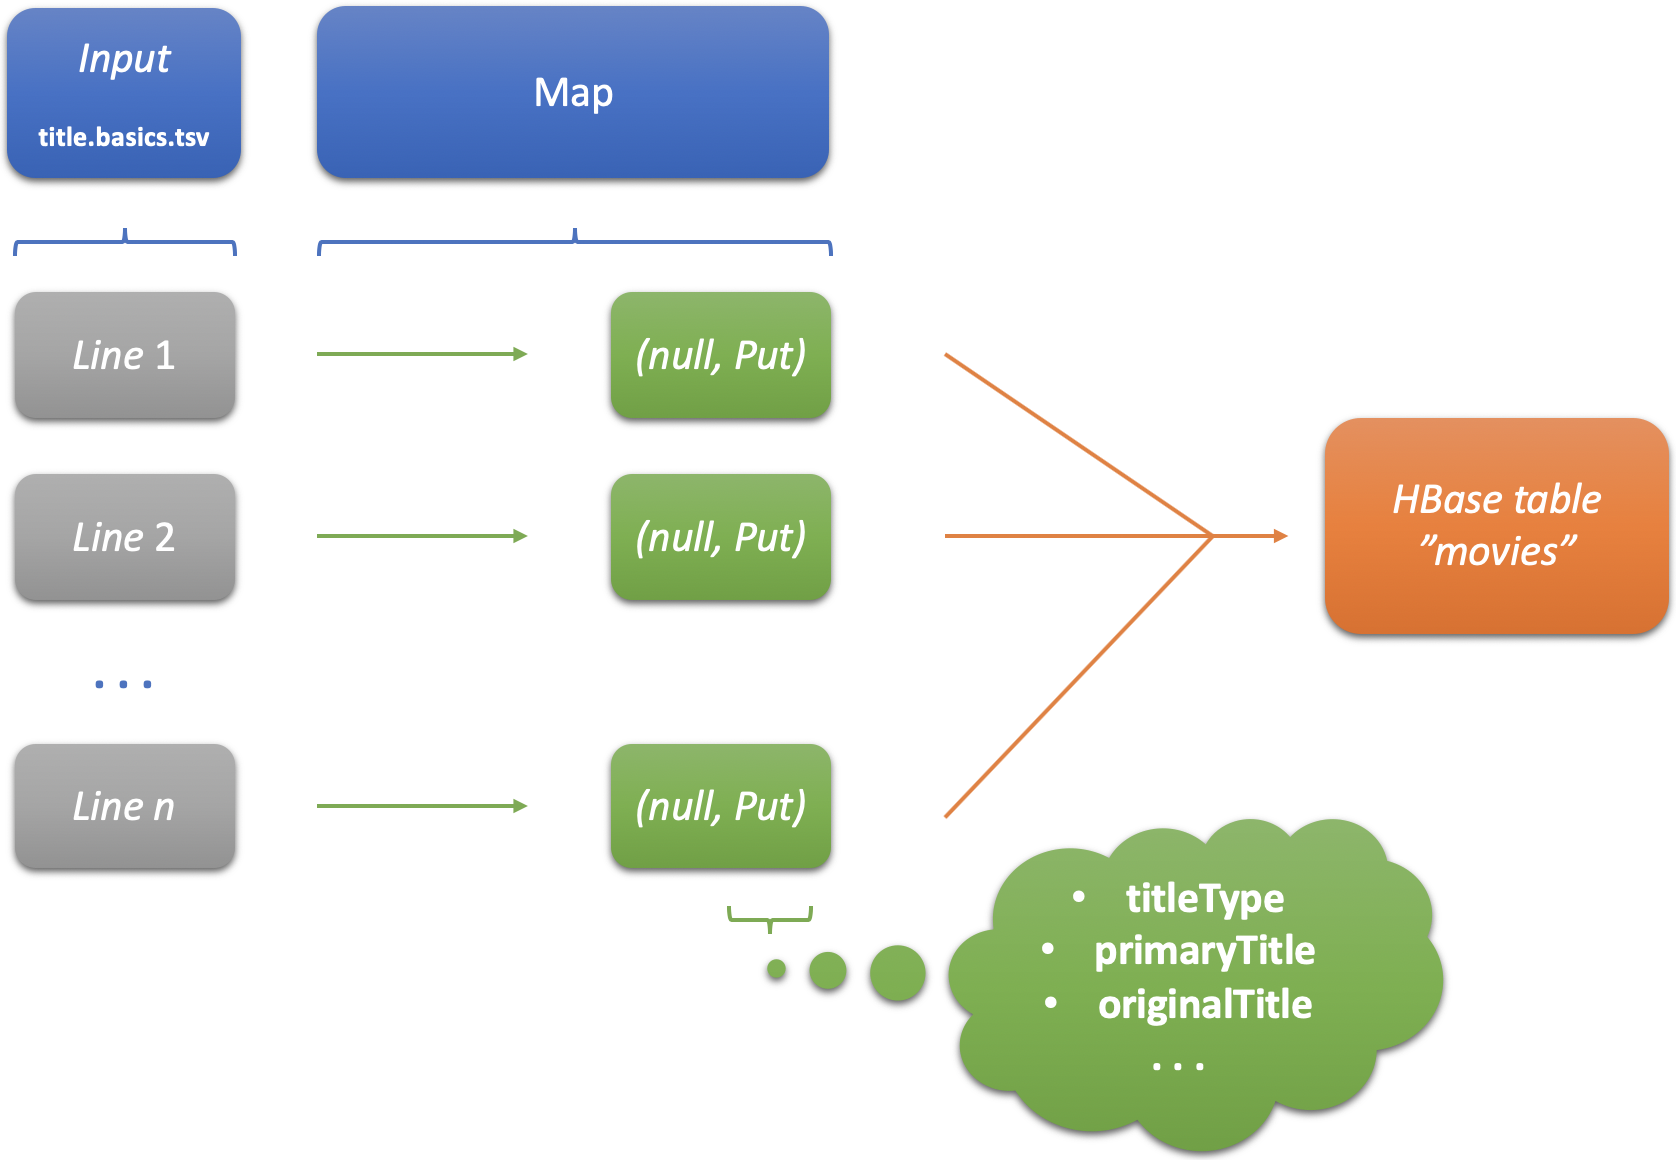
\includegraphics[width=0.64\textwidth]{Imagens/1ª Tarefa - Esquema MapReduce.png}
            \caption{1ª Tarefa - Esquema do paradigma \textit{MapReduce}}
            \label{fig:12}
        \end{figure}


	\section{2ª Tarefa} \label{sec:Task2}
	Tal como foi descrito no início do 2º capítulo deste documento, esta tarefa é composta por 3 alíneas distintas. Como tal é preciso tomar abordagens diferentes de forma a obter resultados corretos para cada uma das mesmas. 
	Após uma leitura cuidadosa sobre o que é pedido em cada uma destas subtarefas, os elementos deste grupo notaram que iria ser necessário recolher 4 dos ficheiros que fazem parte do \textit{dataset IMDB} para extrair os resultados pretendidos.
	Apresenta-se de seguida os 4 ficheiros escolhidos:
	\begin{itemize}
		\item \textit{"name.basics.tsv"}: conjunto de dados caraterísticos de um determinado ator, como por exemplo o seu nome, ano de nascimento, entre outros;
		\item \textit{"title.basics.tsv"}: informação detalhada dos filmes, nomeadamente o ano de começo, géneros, entre outros;
		\item \textit{"title.principals.tsv"}: conjunto de dados relativos aos atores que integram um determinado filme;
		\item \textit{"title.ratings.tsv"}: informação associada à classificação e votação dos filmes presentes na plataforma \textit{IMDB}.
	\end{itemize}
	
	Tal como se pode observar na listagem acima, o formato utilizado para estes ficheiros é o formato \textit{.tsv}. A escolha desta extensão em detrimento de outras é exatamente a mesma que se encontra no início do subcapítulo relativo à \hyperref[sec:Task1]{1ª tarefa}.
	
	À semelhança do que foi indicado nesse mesmo subcapítulo, a execução das soluções desenvolvidas nas secções \hyperref[subsec:Task2-1]{2.3.1} e \hyperref[subsec:Task2-3]{2.3.3} são realizadas com o auxílio do mesmo ficheiro \textit{Dockerfile} com as mesmas opções de execução.
		
		\subsection{Criação da tabela \textit{HBase}} \label{subsec:Task2-1}
		De maneira a criar a tabela \textit{HBase} associada a esta tarefa, foi implementada uma classe \textit{Java}, \textbf{\textit{CreateTableActors}}, que, após conectar-se com a base de dados não relacional \textit{HBase}, trata da sua criação e configuração.
		Durante esse processo, são produzidas duas famílias de colunas, denominadas por \textbf{\textit{details}} e \textbf{\textit{movies}}, onde serão guardados todos os dados pertinentes para esta tarefa. Para além disso, tal como o nome da classe atrás evidencia, foi atribuído o nome \textbf{\textit{actors}} à tabela criada.

		Foi também criada uma classe \textit{Java} extra, \textbf{\textit{DeleteTableActors}}, que trata de eliminar a tabela descrita anteriormente, sempre que for oportuno.
        
        Apresenta-se de seguida o modelo da tabela \textit{HBase} pretendido para a concretização desta tarefa:
        \begin{figure}[H]
            \centering
            \includegraphics[width=1.0\textwidth]{Imagens/2ª Tarefa - Tabela Hbase.png}
            \caption{2ª Tarefa - Modelo da tabela \textit{HBase "actors"}}
            \label{fig:13}
        \end{figure}

			\subsubsection{Alternativa}
			Uma possibilidade válida para realizar todo o processo associado à criação da tabela requerida seria utilizar a \textit{HBase shell} de forma direta. Por forma a aceder a este recurso basta invocar a instrução presente na \hyperref[fig:6]{figura nº 6}.
			Exibe-se de seguida o comando alternativo para realizar a criação da tabela mencionada:

			\begin{figure}[H]
				{
					\color{teal}
					\begin{Verbatim}[commandchars=\\\{\}]
              \textcolor{orange}{hbase(main):001:0>} create "actors", "details", "movies"
					\end{Verbatim}
				}
				\caption{2ª Tarefa : Alternativa - Criação da tabela \textit{HBase "actors"}}
				\label{fig:14}
			\end{figure}
			
			Quanto à remoção da mesma tabela, à semelhança do procedimento tomado para a sua criação, adota-se a estratégia de usufruir explicitamente o mecanismo disponibilizado pela \textit{HBase shell}:
			\begin{figure}[H]
				{
					\color{teal}
					\begin{Verbatim}[commandchars=\\\{\}]
                        \textcolor{orange}{hbase(main):001:0>} disable "actors"
                        \textcolor{orange}{hbase(main):002:0>} drop "actors"
					\end{Verbatim}
				}
				\caption{2ª Tarefa : Alternativa - Remoção da tabela \textit{HBase "actors"}}
				\label{fig:15}
			\end{figure}

		\subsection{Transferência de ficheiros para a plataforma \textit{Hadoop HDFS}} \label{subsec:Task2-2}
		Dado que o ficheiro \textit{"title.basics.tsv"} já foi transferido para a plataforma \textit{Hadoop HDFS} na tarefa anterior, resta apenas transferir os 3 ficheiros restantes, isto é, \textit{"name.basics.tsv"}, \textit{"title.principals.tsv"} e \textit{"title.ratings.tsv"}.
		Antes de mostrar as duas alternativas para proceder à transferência destes 3 ficheiros, é importante salientar que a pasta criada na 1ª tarefa (denominada por \textit{data}) é novamente utilizada para armazenar os mesmos. A instrução associada à criação da mesma pasta encontra-se disponível na \hyperref[fig:9]{figura nº 9}.

			\subsubsection{1ª Alternativa}
			Nesta possibilidade evidencia-se o campo \texttt{source} que corresponde à diretoria da pasta que contém o ficheiro de \textit{input} pretendido.
			Dito isto, apresenta-se agora a primeira alternativa:
			\begin{figure}[H]
				{
					\color{teal}
					\begin{verbatim}
					   docker run --network docker-hbase_default
					              --env-file docker-hbase/hadoop.env
					              --mount type=bind,source="/path/to/local/folder/data",target=/data
					              bde2020/hadoop-base hdfs dfs -put /data/name.basics.tsv /data
								  
					   docker run --network docker-hbase_default
					              --env-file docker-hbase/hadoop.env
					              --mount type=bind,source="/path/to/local/folder/data",target=/data
					              bde2020/hadoop-base hdfs dfs -put /data/title.principals.tsv /data
								  
					   docker run --network docker-hbase_default
					              --env-file docker-hbase/hadoop.env
					              --mount type=bind,source="/path/to/local/folder/data",target=/data
					              bde2020/hadoop-base hdfs dfs -put /data/title.ratings.tsv /data
					\end{verbatim}
				}
				\caption{2ª Tarefa : 1ª Alternativa - Transferência dos 3 ficheiros de \textit{input} para a plataforma \textit{Hadoop HDFS}}
				\label{fig:16}
			\end{figure}

			\subsubsection{2ª Alternativa}
			Esta opção corresponde ao modo interativo de execução disponibilizado pela instrução \textit{docker run}.
			Uma vez feita esta observação, expõe-se a seguir a segunda alternativa:
			\begin{figure}[H]
				{
					\color{teal}
					\begin{verbatim}
					   docker run -it
					              --network docker-hbase_default
					              --env-file docker-hbase/hadoop.env
					              bde2020/hadoop-base bash

					   curl https://datasets.imdbws.com/name.basics.tsv.gz | gunzip |
					   hdfs dfs -put - hdfs://namenode:9000/data/name.basics.tsv

					   curl https://datasets.imdbws.com/title.principals.tsv.gz | gunzip |
					   hdfs dfs -put - hdfs://namenode:9000/data/title.principals.tsv

					   curl https://datasets.imdbws.com/title.ratings.tsv.gz | gunzip |
					   hdfs dfs -put - hdfs://namenode:9000/data/title.ratings.tsv
					\end{verbatim}
				}
				\caption{2ª Tarefa : 2ª Alternativa - Transferência dos 3 ficheiros de \textit{input} para a plataforma \textit{Hadoop HDFS}}
				\label{fig:17}
			\end{figure}

		\subsection{População da tabela \textit{HBase}} \label{subsec:Task2-3}
			Ao contrário do que foi feito na primeira parte deste projeto, foi tomada a decisão de fazer uma separação do trabalho em duas unidades distintas: em primeiro lugar, é inserida a informação relativa aos detalhes pessoais de cada ator (nome e data de nascimento/morte) e, posteriormente, procede-se à inserção dos dados relativos às carreiras dos mesmos (número total de filmes e os 3 filmes com melhor classificação).
			
			\subsubsection{Nome, datas de nascimento e morte do ator} \label{sssec:Task2-3-1}
			Para a população da tabela criada com a informação relativa ao nome e data de nascimento/morte de cada ator, foi implementada uma classe \textit{Java}, à qual foi dada a designação de \textbf{\textit{Actor2Details}}.
			Esta classe utiliza uma versão simplificada do paradigma \textit{MapReduce}, pois apenas é executada a fase de \textit{map}.
			Nesta fase única, são processadas as linhas do ficheiro \textit{"name.basics.tsv"}, previamente inserido na plataforma \textit{Hadoop HDFS}, escolhendo a informação relevante e inserindo o resultado pretendido na tabela \textit{actors}.
			\begin{figure}[H]
				\centering
				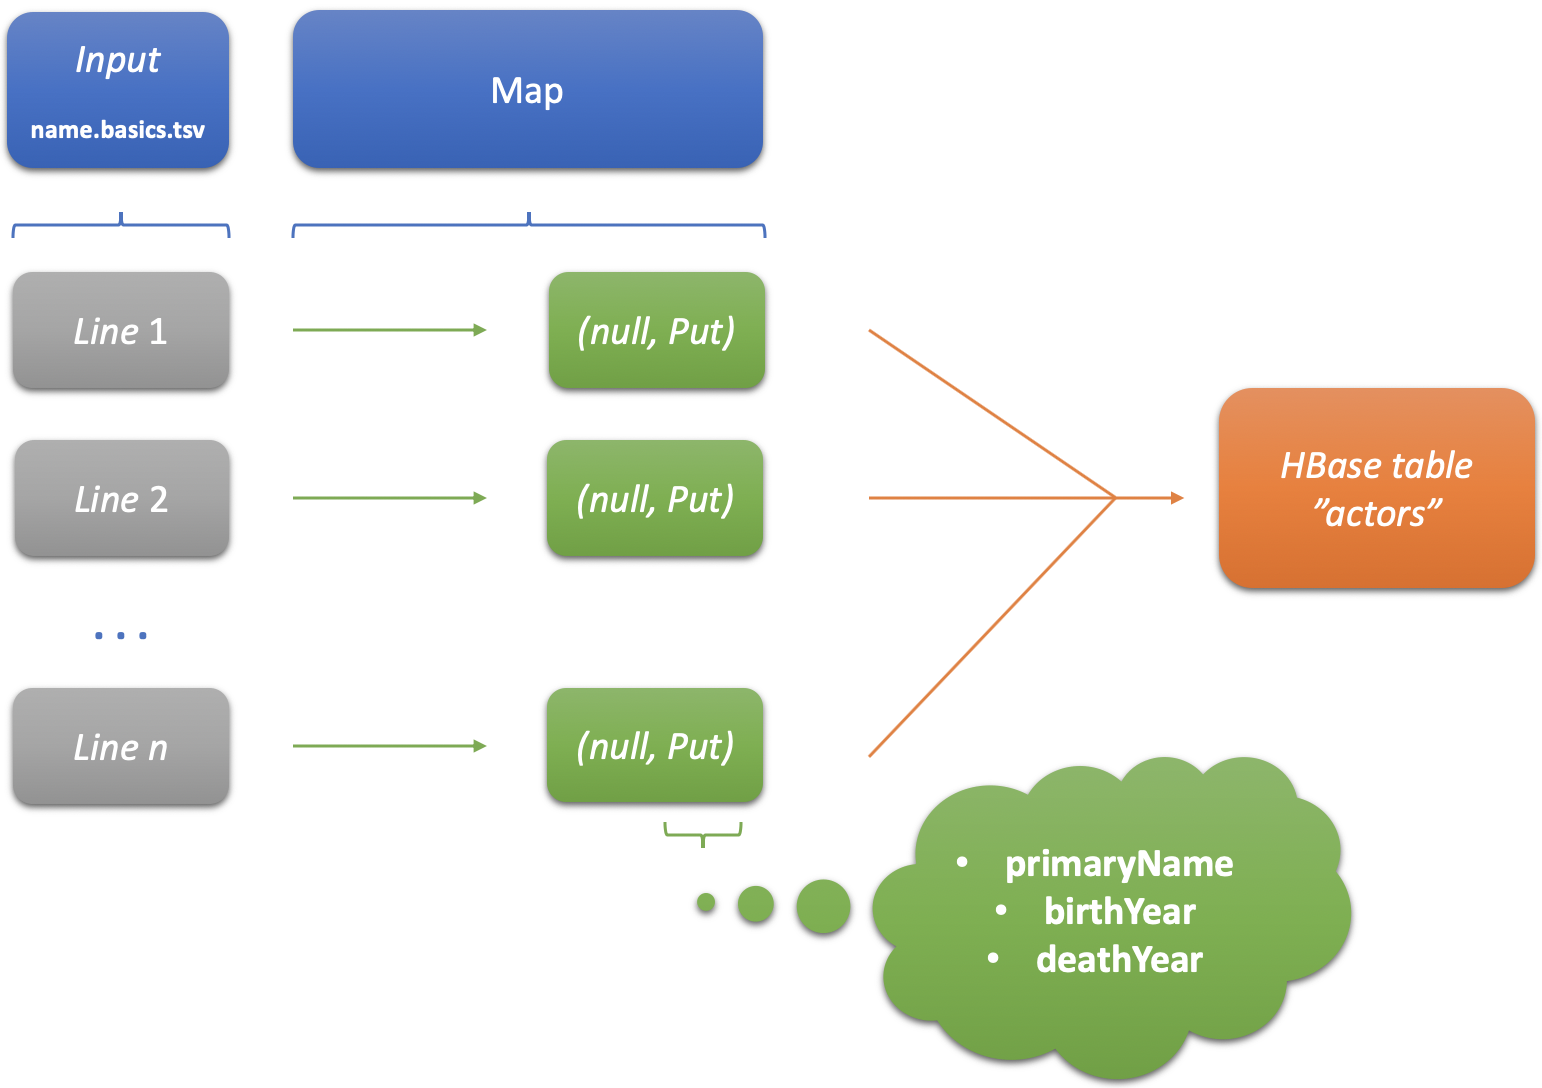
\includegraphics[width=0.58\textwidth]{Imagens/2ª Tarefa - Actor2Details - Esquema MapReduce.png}
				\caption{2ª Tarefa - \textit{Actor2Details} - Esquema do paradigma \textit{MapReduce}}
				\label{fig:18}
			\end{figure}

			\subsubsection{Número total de filmes + Top 3} \label{sssec:Task2-3-2}
			Por último, para completar a informação relativa a cada ator, foi criada uma classe denominada por \textbf{\textit{Actor2Movies}}. Esta classe consiste na execução de duas tarefas \textit{MapReduce} sobre os dados dos ficheiros presentes no \textit{Hadoop HDFS} e dos dados contidos na tabela gerada no primeiro exercício.
			
			Passando à primeira tarefa, esta tem como responsabilidade a geração de pares \textit{(nconst, (originalTitle, averageRating))}, em que \textit{nconst} é o identificador do ator, \textit{originalTitle} representa o título de um filme em que esse ator participou e \textit{averageRating} a classificação média desse mesmo filme.
			
			Para atingir este objetivo, são efetuadas três sub-tarefas \textit{map}, a que são dados os nomes \textit{Left}, \textit{Middle} e \textit{Right}, como é habitual em execuções deste tipo. Falando de cada uma em particular, temos que a \textit{Left} toma como entrada o conteúdo do ficheiro \textit{"title.principals.tsv"} e gera um par \textit{(tconst, (L, nconst))} para cada ator \textit{nconst} que participou no filme \textit{tconst}. A \textit{Middle} extrai os dados da tabela criada no primeiro exercício, com a informação de cada filme, e cria pares \textit{(tconst, (M, originalTitle))}, ou seja, a cada identificador de um filme associa o seu título original. Temos ainda a \textit{Right}, que, a partir dos conteúdos do ficheiro \textit{"title.rating.tsv"}, associa a cada identificador de um filme a respetiva classificação \textit{(tconst, (R, averageRating))}.
			Note-se que as letras \textit{L}, \textit{M} e \textit{R} são prefixadas ao conteúdo das variáveis correspondentes.
			
			Como nesta fase de \textit{map} a chave de cada par resultante é o identificador do filme \textit{tconst}, quando se passa à fase \textit{reduce} temos a garantia que, para um dado filme, o seu título, todos os atores que nele participaram e a sua classificação estarão associados à sua chave. Assim, o nosso \textit{reducer} consiste na escrita, para um \textit{sequence file}, de associações do tipo \textit{(nconst, (originalTitle, averageRating))}, ou seja, para cada ator é introduzida uma destas linhas por cada filme em que participou.

			Tal como o docente desta disciplina sugeriu durante a realização do guião nº 4, optou-se por utilizar um \textit{sequence file} em detrimento de um simples ficheiro de texto. Esta decisão recai sobretudo no facto deste tipo de ficheiro se encontrar serializado, no formato binário, em pares chave-valor e, para além disso, ser consideravelmente mais rápido na execução de operações de leitura e escrita de dados.
			\begin{figure}[H]
				\centering
				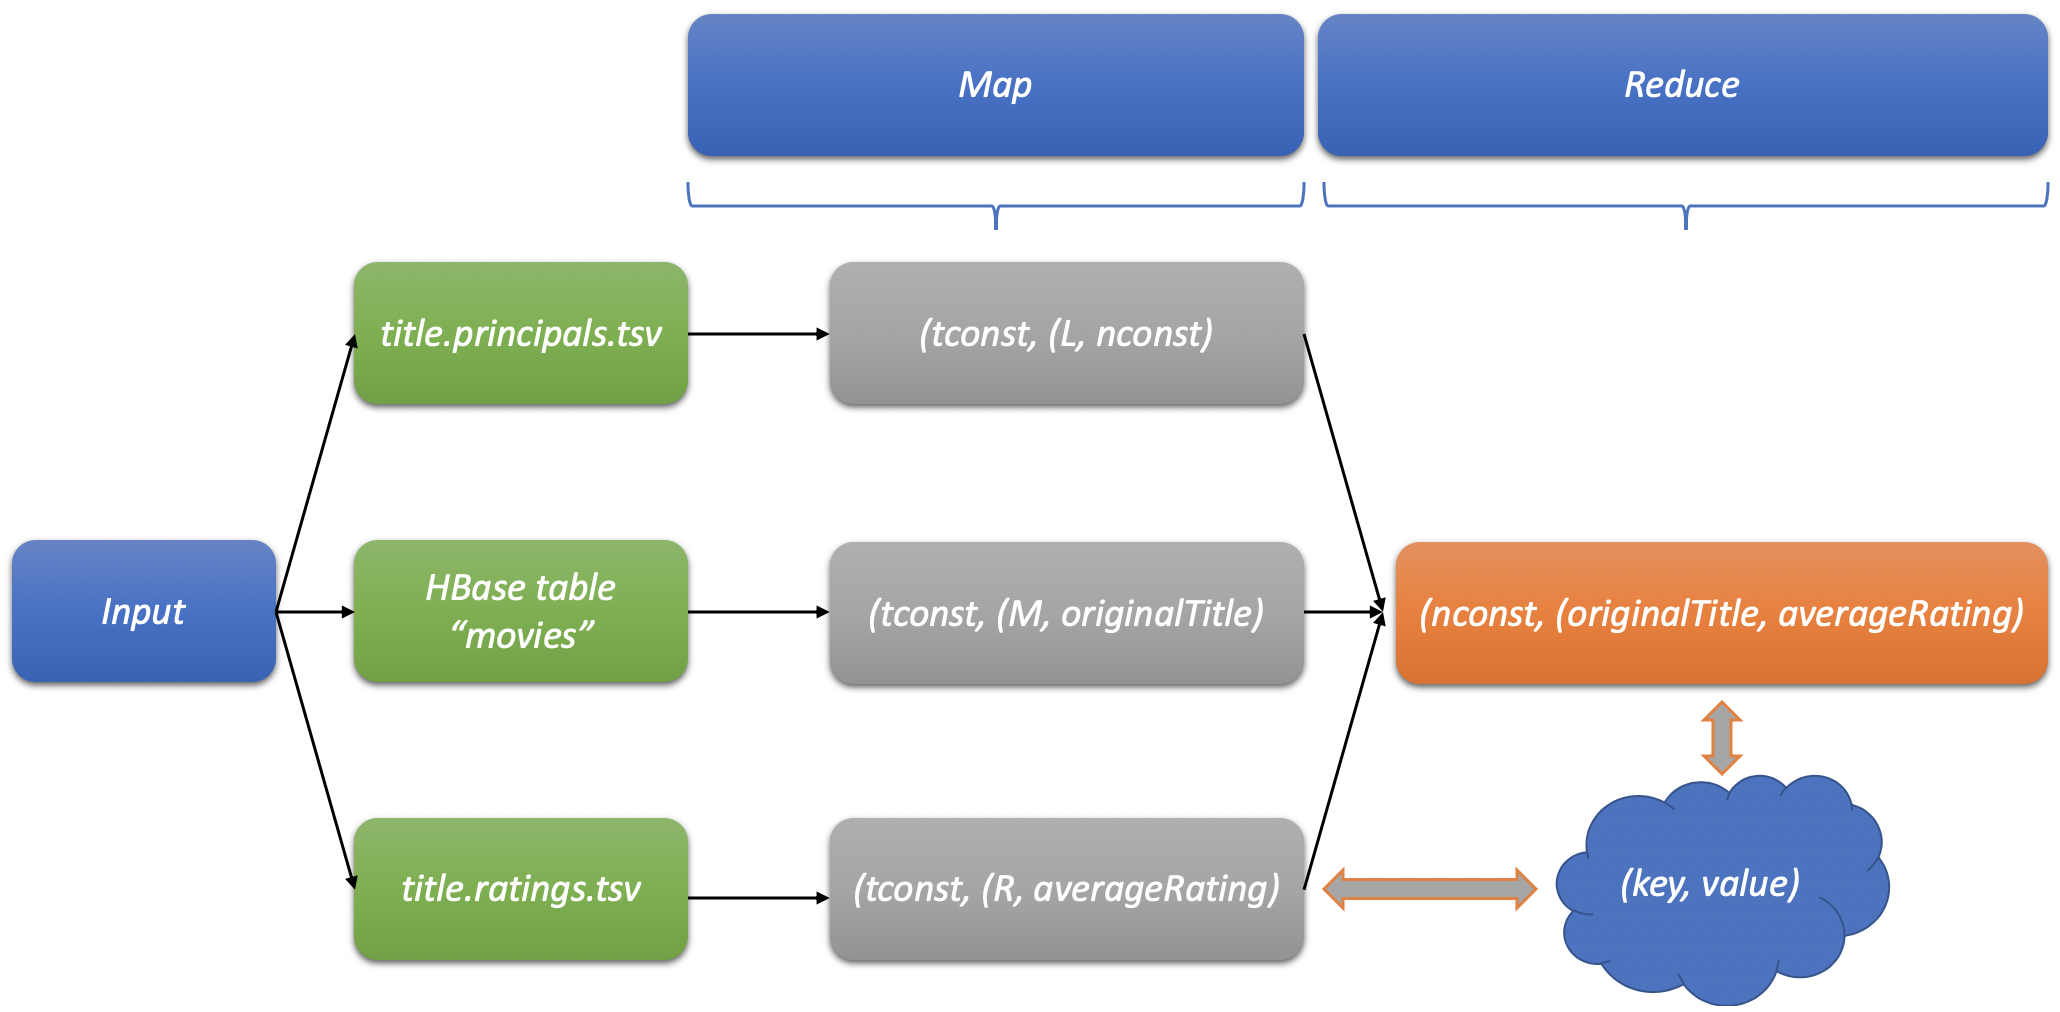
\includegraphics[width=0.9\textwidth]{Imagens/2ª Tarefa - Actor2Movies - 1º Esquema MapReduce.png}
				\caption{2ª Tarefa - \textit{Actor2Movies} - 1º Esquema do paradigma \textit{MapReduce}}
				\label{fig:19}
			\end{figure}

			Estando esta informação armazenada no \textit{HDFS} num \textit{sequence file}, resta apenas executar uma outra tarefa \textit{MapReduce} para inserir os dados na tabela \textit{HBase actors}.
			
			Como os dados foram tratados na tarefa anterior, na fase de \textit{map} é apenas necessário passar a informação tal como está para a fase de \textit{reduce}. É aqui, tendo em conta que a cada ator está associada uma lista de pares \textit{(originalTitle, averageRating)}, que será calculado o número de filmes de cada ator e a lista dos 3 melhores filmes. estando os dados previamente processados, isto torna-se trivial, sendo apenas necessário ver o comprimento desta lista para obter o número de filmes do ator e ordenar os mesmos por classificação, escolhendo os primeiros 3. Com vista a tornar a execução determinista, tivemos o cuidado de, em caso de empate na classificação, escolhermos os filmes por ordem alfabética.
			
			Por fim, os dados são inseridos na tabela pretendida.
			\begin{figure}[H]
				\centering
				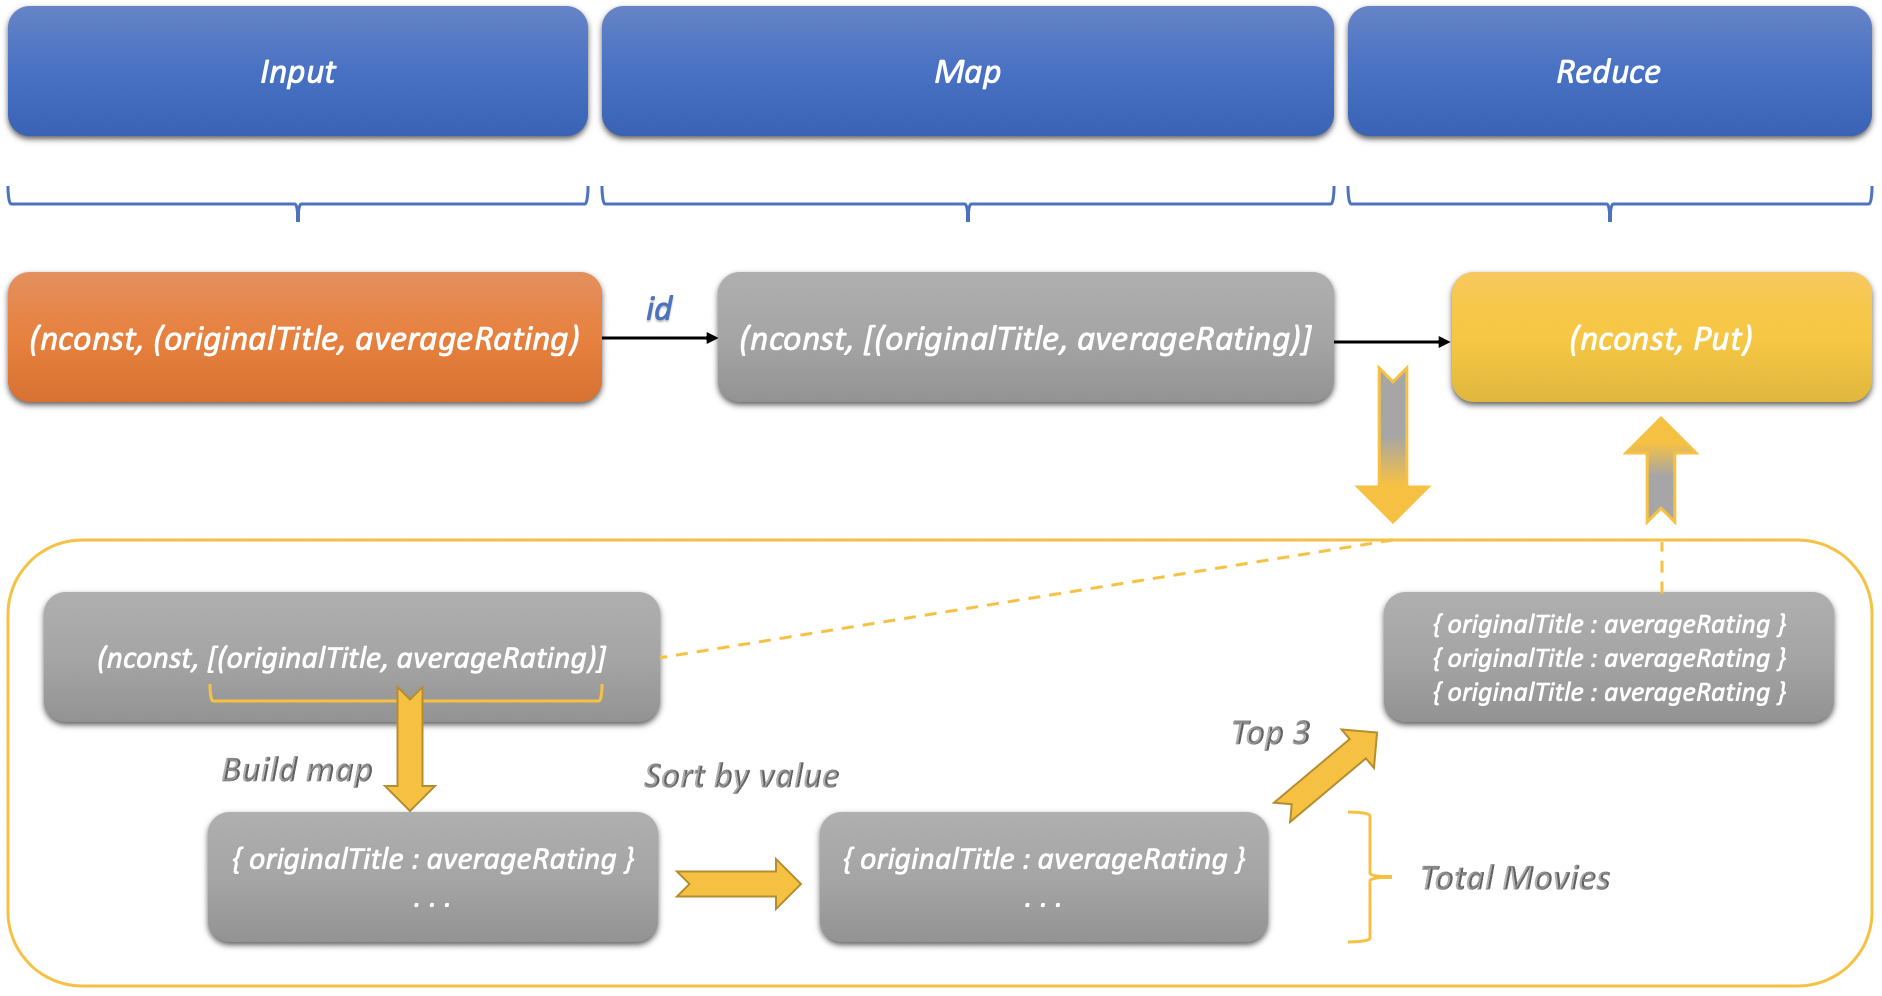
\includegraphics[width=0.9\textwidth]{Imagens/2ª Tarefa - Actor2Movies - 2º Esquema MapReduce.png}
				\caption{2ª Tarefa - \textit{Actor2Movies} - 2º Esquema do paradigma \textit{MapReduce}}
				\label{fig:20}
			\end{figure}
}

\chapter{Conclusão} \label{ch:Conclusion}
\large{
	Para concluir, temos a referir que este trabalho foi bastante enriquecedor e muito provavelmente representativo de uma tarefa comum de Cientistas de Dados para processamento e armazenamento de informação resultante da observação de diversas fontes.
	Tivemos a oportunidade de utilizar o paradigma \textit{MapReduce} do \textit{Hadoop} e ainda o sistema de ficheiros \textit{HDFS}. Estas ferramentas, por estarem orientadas para este tipo de tarefas, foram indicadas para este trabalho. Apesar disso, pudemos constatar alguns problemas, pois não nos é dada liberdade total nas operações que queremos efetuar sobre os dados. Um exemplo, é a imposição de termos de ter uma tarefa de \textit{map}, mesmo que tal não seja necessário. Outro, é a obrigatoriedade de escrever os dados para disco entre duas tarefas.
	Como vimos nas aulas, desde a criação do \textit{MapReduce} do \textit{Hadoop} surgiu o \textit{Spark}, que nos dá muito mais liberdade no tipo e ordem das operações que queremos realizar.
}

\appendix
\chapter{Observações} \label{ch:Observations}
\begin{itemize}
    \item Documentação \textit{Java} 8:
    \par \textit{\url{https://docs.oracle.com/javase/8/docs/api/}}
	\item \textit{Maven}:
    \par \textit{\url{https://maven.apache.org/}}
    \item \textit{Hadoop}:
    \par \textit{\url{https://hadoop.apache.org/}}
    \item \textit{HBase}:
    \par \textit{\url{https://hbase.apache.org/}}
\end{itemize}

\end{document}